\documentclass[12pt]{article}
\usepackage[utf8]{inputenc}
\usepackage[
a4paper,		% papel A4
left=2cm,		% margem esquerda
right=2cm,		% margem direita
top=2cm,		% margem superior
bottom=2cm		% margem inferior
]{geometry}
\usepackage[T1]{fontenc}	
\usepackage{array,latexsym,amssymb}
\usepackage{amsmath,amsfonts,amssymb,amsthm,mathabx,amstext}
\usepackage{dsfont}	% Conjuntos: $\mathds{N, Z, Q, R, C}$
\usepackage{graphicx}
\begin{document}
\begin{center}
	UNIVERSIDADE FEDERAL DA PARAÍBA\\
	Introdução à Álgebra Linear\\
	Segunda Prova\\
	Paulo Ricardo Seganfredo Campana - 20210044220\\
\end{center}

\noindent Questão 1.\\

\noindent a) Uma transformação que satisfaz as propriedades:\\

$T(u+v)=T(u)+T(v)$ e $T(\alpha u)=\alpha T(u)\quad\forall\alpha\in\mathds{R}\quad\forall u,v\in V$\\

\noindent b)\\
\noindent I) 

$T(0,0)=(0\cos0)=(0,1)$\hfill $T(0,0)\neq0$ portanto não é linear.
%Seja $u=(u_{1},u_{2})$ e $v=(v_{1},v_{2})$\\
%$T(u+v)=T(u_{1}+v_{1},u_{2}+v_{2})=(u_{1}+v_{1},\cos(u_{2}+v_{2}))=$\\
%$(u_{1},\cos(u_{2}))+(v_{1},\cos(v_{2}))=T(u_{1},u_{2})+T(v_{1},v_{2})=T(u)+T(v)$\\
%$T(\alpha u)=T(\alpha u_{1},\alpha u_{2})=(\alpha u_{1}, \cos(\alpha %u_{2}))\neq\alpha(u_{1},\cos(u_{2}))$\hfill Portanto não é linear.\\

\noindent II)\\

$T(ax^{2}+bx+c+dx^{2}+ex+f)=T((a+d)x^{2}+(b+e)x+(c+f))=$\\

$(a+d)x^{2}+(-2a-2d+b+e)x+(a+d-b-e+c+f)=$\\

$(ax^{2}+(-2a+b)x+(a-b+c))+(dx^{2}+(-2d+e)x+(d-e+f))=T(ax^{2}+bx+c)+T(dx^{2}+ex+f)$\\

$T(\alpha ax^{2}+\alpha bx+\alpha c)=(\alpha ax^{2}+\alpha(-2a+b)x+\alpha(a-b+c))=$\\

$\alpha(ax^{2}+(-2a+b)x+(a-b+c))=T(ax^{2}+bx+c)$\hfill Portanto é linear.\\

\noindent III) Sem perda de generalidade para o caso $2x2$:\\

$T\left(\begin{bmatrix}a&b\\c&d\end{bmatrix}+\begin{bmatrix}e&f\\g&h\end{bmatrix}\right)=T\left(\begin{bmatrix}a+e&b+f\\c+g&d+h\end{bmatrix}\right)=\begin{bmatrix}a+e&c+g\\b+f&d+h\end{bmatrix}=\begin{bmatrix}a&c\\b&d\end{bmatrix}+\begin{bmatrix}e&g\\f&h\end{bmatrix}=$\\

$T\left(\begin{bmatrix}a&b\\c&d\end{bmatrix}\right)+\left(\begin{bmatrix}e&f\\g&h\end{bmatrix}\right)$\\

$T\left(\alpha\begin{bmatrix}a&b\\c&d\end{bmatrix}\right)=T\left(\begin{bmatrix}\alpha a&\alpha b\\\alpha c&\alpha d\end{bmatrix}\right)=\begin{bmatrix}\alpha a&\alpha c\\\alpha b&\alpha d\end{bmatrix}=\alpha\begin{bmatrix}a&c\\b&d\end{bmatrix}=$\\

$\alpha T\left(\begin{bmatrix}a&b\\c&d\end{bmatrix}\right)$\hfill Portanto é linear.\\

\noindent Questão 2.\\



$x(1,2,0,-4)+y(2,0,-1,3)+z(a,b,c,d)=(x+2y+az,2x+bz,-y+cz,-4x+3y+dz)$\\

$T(x,y,z)=(x+2y+az,2x+bz,-y+cz,-4x+3y+dz)$\\

\noindent Questão 3.\\

\noindent I)\\

Seja $v\in N(T)$, $T(v)=0$, porém $T(0)=0$, já que $T$ é injetora, apenas um vetor pode valer $0$, $v=0$ ou seja $N(T)=\lbrace0\rbrace$.\\

\noindent II)\\

Pelo teorema de dimensão: $dimN + dimIm = dimV\longrightarrow dimIm = dimV\longrightarrow Im(T)=V$\\

\noindent III)\\

Foi visto anteriormente que se $Im(T)=V\longrightarrow N(T)=\lbrace0\rbrace$ e que se $N(T)=\lbrace0\rbrace\longrightarrow T$ é injetora, portanto se $Im(T)=V\longrightarrow T$ é injetora.\\

\noindent Questão 4.\\

\noindent I)\\

$\begin{bmatrix}-9&4&4\\-8&3&4\\-16&8&7\end{bmatrix}~\begin{bmatrix}-9&4&4\\-8&3&4\\0&2&-1\end{bmatrix}~\begin{bmatrix}-9&12&0\\-8&11&0\\0&2&-1\end{bmatrix}~\begin{bmatrix}8&-\frac{32}{3}&0\\-8&11&0\\0&2&-1\end{bmatrix}~\begin{bmatrix}0&-\frac{1}{3}&0\\-8&11&0\\0&2&-1\end{bmatrix}$\\

$y=0,\quad z=0,\quad x=0\longrightarrow N(T)=\lbrace0,0,0\rbrace$\\

$Im(T)=\mathds{R}^{3}$ pois $N(T)=\lbrace0,0,0\rbrace$ como visto na demonstração na questão 3.\\

Portanto é injetora e sobrejetora, ou seja, bijetora, e caracteriza isomorfismo.\\

$\begin{bmatrix}-9&4&4\\-8&3&4\\-16&8&7\end{bmatrix}^{-1}=\begin{bmatrix}\frac{-11}{3}&\frac{4}{3}&\frac{4}{3}\\\frac{-8}{3}&\frac{1}{3}&\frac{4}{3}\\\frac{-16}{3}&\frac{8}{3}&\frac{5}{3}\end{bmatrix}$\\

$T^{-1}(x,y,z)=\dfrac{1}{3}(-11x+4y+4z,-8x+y+4z,-16x+8y+5z)$\\

\noindent II)\\

$det\begin{vmatrix}-9-\lambda&4&4\\-8&3-\lambda&4\\-16&8&7-\lambda\end{vmatrix}=0$\\

$(-9-\lambda)(3-\lambda)(7-\lambda)-256-256+64(3-\lambda)-16(-9-\lambda)+32(7-\lambda)$\\

$-\lambda^{3}+\lambda^{2}+5\lambda+3=-(\lambda+1)^{2}(\lambda-3)\quad\lambda=\lbrace-1,3\rbrace$\\

$\lambda=-1\quad\begin{vmatrix}-8&4&4\\-8&4&4\\-16&8&8\end{vmatrix}\quad y+z=x\hfill v=(y+z,y,z)=y(1,1,0)+z(1,0,1)$\\

$\lambda=3\quad\begin{vmatrix}-12&4&4\\-8&0&4\\-16&8&4\end{vmatrix}\left\{\begin{array}{@{}l@{}}4z=8x\longrightarrow z=2x\\-16x+8y+4z=0\longrightarrow-8x+8y=0\longrightarrow x=y\end{array}\right.\hfill v=x(1,1,2)$

Os três autovetores geram o $\mathds{R}^{3}$ portanto $T$ é diagonalizável.\\

\noindent Questão 5.\\

\noindent I) Verdadeiro, pois isso significa que o polinômio característico/minimal é da forma $(x_{1}-\lambda_{1})(x_{2}-\lambda_{2})\dots(x_{n}-\lambda_{n})$ com todos os $\lambda$s distintos, que pelo teorema 3.3.3 da 3ª unidade, é dito como diagonalizável.\\

\noindent II) Verdadeiro, segue a demonstração do material da 3ª unidade.\\

\begin{figure}[h!]
	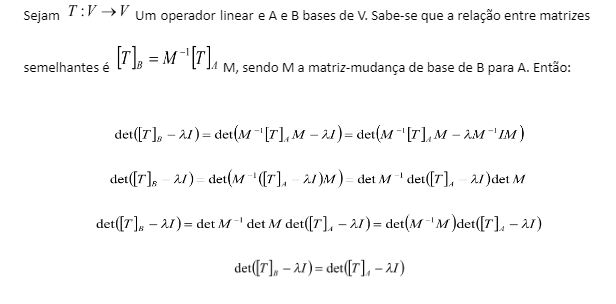
\includegraphics[scale=0.8]{q5b}
\end{figure}

\noindent III) Verdadeiro, sem perda de generalização para o caso de 2 autovalores:\\

Seja $T(v_{1})=\lambda_{1}v_{1}$ e $T(v_{2})=\lambda_{2}v_{2}$ e $\lambda_{1}\neq\lambda_{2}$\\

$a_{1}v_{1}+a_{2}v_{2}=0\qquad\qquad a_{1}T(v_{1})+a_{2}T(v_{2})=0$\\

$a_{1}\lambda_{1}v_{1}+a_{2}\lambda_{2}v_{2}=0\qquad\qquad a_{1}\lambda_{1}v_{1}+a_{2}\lambda_{1}v_{2}=0\qquad\qquad a_{2}(\lambda_{2}-\lambda_{1})v_{2}=0$\\

Já que $\lambda_{1}-\lambda_{2}\neq0$ e $v\neq0$, $a_{2}=0$, o mesmo vale para $a_{1}$\\

Portanto a única solução para $a_{1}v_{1}+a_{2}v_{2}=0$ é a trivial $a_{1}=a_{2}=0$ e $v_{1},v_{2}$ são LI.\\

\noindent IV) Verdadeiro.\\

$det\begin{vmatrix}0-\lambda&0&\cdots&0\\0&0-\lambda&\cdots&0\\\vdots&\vdots&\ddots&\vdots\\0&0&\cdots&0-\lambda\end{vmatrix}=0\qquad -\lambda^{n}=0$\\

Porém a função exponencial $-\lambda^{n}$ não possui raiz, não existe autovalores então não pode ser diagonalizável.\\





















\end{document}